\section{Estructura general}

    El laboratorio virtual de sistemas de control clásicos y difusos fue pensado de modo que cada una de sus funcionalidades principales sean independientes la una de la otra, no obstante, ciertas rutinas son comunes entre ellas. Por otro lado, se organizo la aplicación de modo que cada funcionalidad principal posea un archivo \enquote{handler}, el cual hará de intermediario entre la interfaz gráfica y las rutinas de calculo que se encuentran en un archivo de rutinas. La \cref{fig:estructuraMain} sirve como referencia de la estructura general utilizada.

    \begin{figure}[htb]
        \centering
        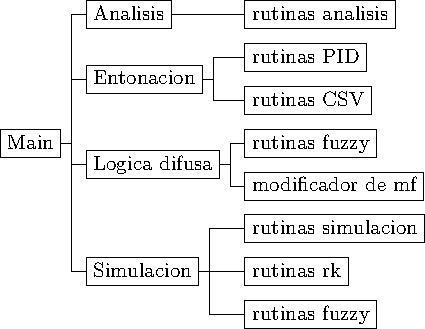
\includegraphics[width=0.6\textwidth]{estructuraMain.pdf}
        \caption[Diagrama general de la aplicación]{\textbf{Diagrama general de la aplicación}. La estructura general de la aplicación, la segunda columna representa a los archivos handler mientras que la tercera son los archivos de rutinas  Fuente: Elaboración propia.} 
        \label{fig:estructuraMain}
    \end{figure}

\section{Análisis de sistemas de control}
    
    Con esta función se quiso dar la posibilidad de realizar los análisis en el tiempo y en frecuencia típicos para un proceso ingresado por el usuario, los análisis típicos son: respuesta al escalón, respuesta al impulso, diagrama de bode, diagrama de Nyquist, lugar de las raíces y diagrama de Nichols. El \cref{code:analisis} muestra un pseudo código de la funcionalidad de análisis de sistemas de control.

    \begin{longlisting}
        \caption{Pseudo código para el análisis de sistemas de control}
        \label{code:analisis}				
        \begin{minted}[escapeinside=||,
            mathescape=true,
            autogobble=true,
            fontsize=\footnotesize,
            obeytabs=true,
            tabsize=4,
            baselinestretch=1]{text}
            |\bf{WHILE}| True: # Ciclo principal
                |$\vdots$|
                |\bf{IF}| validaciones_entradas_análisis:
                    validar_entradas_análisis()
                
                |\bf{IF}| usuario_presiona_calcular:
                    chequeo_TF_SS()
                    creación_proceso()
                    escalón()
                    impulso()
                    bode()
                    nyquist()
                    lugar_de_las_raíces()
                    nichols()
                    datos()
                |$\vdots$|
        \end{minted}
    \end{longlisting}

    \subsection{Definición del proceso}

        Un proceso deberá ser ingresado para poder realizar el análisis, la entonación o la simulación del mismo. El sistema puede ser definido con los coeficientes del numerador y el denominador de la función de transferencia o puede ser definido ingresando las matrices A, B, C y D de la ecuación de espacio de estados. En ambos casos se deben cumplir con los principios matemáticos que correspondan, i.g., las función de transferencia no puede ser impropia.

    \subsubsection{Tiempo discreto}

        La opción de discretizacion permite llevar el proceso ingresado en tiempo continuo a una aproximación en tiempo discreto con solo ingresar el periodo de muestreo y seleccionar el método a utilizar. Se implementaron los siguientes métodos de discretizacion:

        \begin{enumerate}[leftmargin=\parindent]
            \item Retensor de orden cero  (ZOH)
            \item Retensor de primer orden (FOH)
            \item Euler hacia atrás (backward\_diff)
            \item Euler hacia adelante (Euler)
            \item Transformacion trapezoidal (tustin)
            \item Transformacion matched (matched)
            \item Transformacion de impulso (impulse)
        \end{enumerate}

    \subsubsection{Proceso con atraso o delay}
        
        A los procesos ingresados se les puede agregar un atraso, este atraso es manejado de forma distinta dependiendo de la funcionalidad. Para el caso de la funcionalidad de análisis, el delay fue implementado para la respuesta escalón y la respuesta impulso como un desplazamiento en el tiempo equivalente al delay ingresado, para la respuesta en frecuencia se multiplico $e^{-j\omega \alpha}$ a cada una de las evaluaciones de frecuencia con $\alpha$ como el delay ingresado por el usuario. Para el caso del lugar de las raíces, el delay es implementado utilizando una aproximación por PADE de orden 10.

    \subsection{Respuesta al escalón y al impulso}
        
        La respuesta al escalón, al igual que el resto de análisis implementados, fue realizado utilizando la librería de control para Python. La respuesta impulso se realizo del mismo modo, siendo la entrada al proceso la única diferencia respecto a la respuesta escalón.

    \subsection{Diagrama de Bode}
        
        El diagrama de Bode es realizado también con la librería de control, adicionalmente, fue implementado el calculo de los margenes de ganancia y de fase. La implementación fue realizada desde cero debido a los resultados inaceptables obtenidos con la implementación de la librería de control. El código para el calculo de los margenes de ganancia y fase se puede observar en el \ref{anexo:A}.
        
        